\chapter{Kết luận}
\section{Kết quả đạt được}
\begin{figure}[!hbt]
\begin{center}
    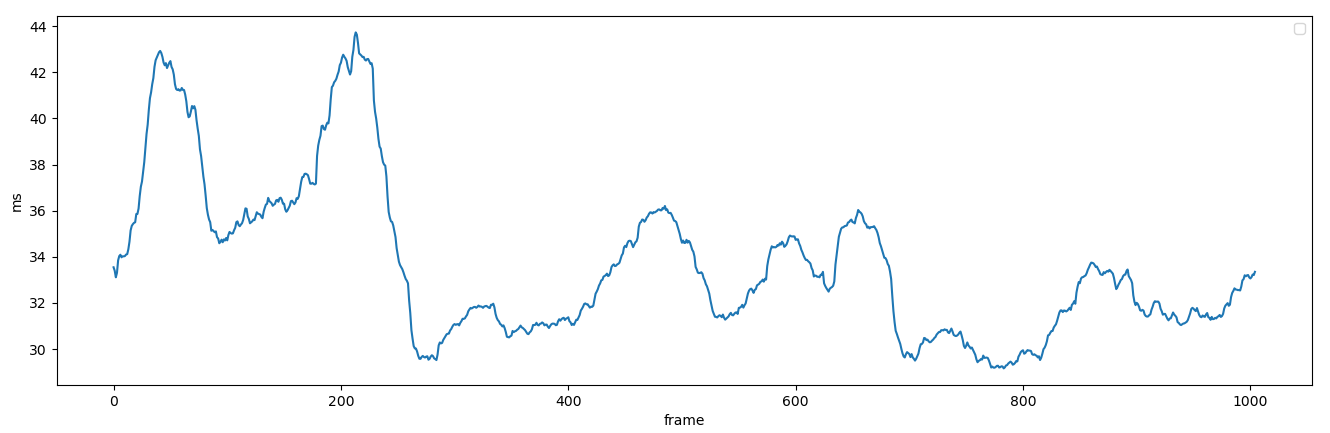
\includegraphics[width=16cm]{img/5_Conclusion/performane_plot_2.png}
    \caption{Thời gian thực thi của hệ thống}
\end{center}
\end{figure}
\begin{itemize}
    \item Trong biểu đồ trên, đường màu cam đại diện cho model AI và xanh đại diện cho khối backend. Ta dễ thấy thời gian xử lý tối thiểu cho 1 frame không quá 30ms nếu frame đó không là frame chứa lỗi/nhiễu. Tuy nhiên, nếu frame đó là frame lỗi, thời gian thực thi có thể lên đến 40ms cho 1 frame. Nhóm sẽ nghiên cứu cải thiện để tìm ra cách tối ưu nhất để cho ra kết quả tối ưu cuối cùng.
    \item Robot có khả năng tuân thủ làn đường, di chuyển với tốc độ trung bình mà không lệch hướng.
    \item Bộ điều khiển PID của hệ thống đã duy trì vị trí chính xác và ổn định trên làn đường
    \item Khi phát hiện có nguy cơ lệch khỏi làn đường, hệ thống sẽ kịp thời đưa ra cảnh báo nguy cơ lệch khỏi làn đường.
    
\end{itemize}
\section{Khó khăn gặp phải}
Có thể thấy, dù hệ thống hoạt động tương đối tốt, robot có khả năng chạy đủ ổn định để hoàn thành kịch bản demo và đạt được mục tiêu đề ra, tuy nhiên vẫn còn một số vấn đề còn tồn đọng như sau:
\begin{enumerate}
    \item \textbf{Khối nhận diện làn đường:}
    \begin{itemize}
        \item 
        \item 
    \end{itemize}
    \item \textbf{Khối bám làn đường:} Module hiện tại chỉ dựa vào chỉ một thông số độ lệch làn đường duy nhất và vẫn chưa ổn định vì cũng chỉ điều khiển mỗi tốc độ góc của TurtleBot3
\end{enumerate}